\documentclass[12pt]{article}

\usepackage[utf8]{inputenc}
\usepackage[english]{babel}

\usepackage{amsmath}
\usepackage{amsfonts}
\usepackage{graphicx}
\usepackage{float}
\usepackage{listings}
\usepackage{subfig}
\usepackage{hyperref}

\usepackage{multirow}

\usepackage{xcolor}

\definecolor{codegreen}{rgb}{0,0.6,0}
\definecolor{codegray}{rgb}{0.5,0.5,0.5}
\definecolor{codepurple}{rgb}{0.58,0,0.82}
\definecolor{backcolour}{rgb}{0.95,0.95,0.92}

\lstdefinestyle{mystyle}{
    backgroundcolor=\color{backcolour},   
    commentstyle=\color{codegreen},
    keywordstyle=\color{magenta},
    numberstyle=\tiny\color{codegray},
    stringstyle=\color{codepurple},
    basicstyle=\ttfamily\footnotesize,
    breakatwhitespace=false,         
    breaklines=true,                 
    captionpos=b,                    
    keepspaces=true,                 
    numbers=left,                    
    numbersep=5pt,                  
    showspaces=false,                
    showstringspaces=false,
    showtabs=false,                  
    tabsize=2
}

\lstset{style=mystyle}

\newcommand{\qed}{\hfill \ensuremath{\Box}}
\newcommand{\bbeta}{\vec{\beta}} 
\newcommand{\hes}{X^TX} 


% TODO: REWRITE ALL COST FUNCTIONS TO INDEX, NOT LINEAR ALGEGBRA

% TODO: Discuss removing the mean / rescaling

% TODO: Add discussion on scaling the data
        
\begin{document}
\begin{titlepage}
   \begin{center}
        \vspace{2cm}

        {\LARGE \textbf{Project 1}}

        \vspace{3em}

        Herman Brunborg


        \vspace{0.5em}

        FYS-STK4155

        \vspace{0.5em}

        University of Oslo

        \vfill

        \today
   \end{center}
\end{titlepage}

\tableofcontents

\newpage

\begin{abstract}
    % TODO: ADD ACTUAL FINDINGS
    In this article the we will study three linear regression methods, more precisely the ordinary least squares (OLS) regression, Ridge regression and Lasso regression, for sampeling both the Franke Function and for real terrain data. 

    For accessing the performance of the models, we have calculated mean squared error (MSE), R2 scores, bias and variance using bootstrap and looked at k-fold cross validation and bootstrap as resampeling techniques.

    The goals for the project were to check which model has the best and most stable performance.

    The main findings are that linear regression models can be very powerful, being able to fit complex data with the ability to save models much more space efficiently than that of saving the data raw.

    Among the three linear regression models tested, ridge regression seems to have the best performance, but this does not mean it is always the correct or best choice.
\end{abstract}

\section{Introduction}

In data science and statistics, one of the main aims is to explain or predict some output based on some input. This is done by fitting a model which one hopes will fit the underlying data. One such method is linear regression.

In linear regression, we try to approximate a model for the relationship between some input and output data using linear parameters.
The main usecases of linear regression are for predicting the behaviour of new data, or to analyse the correlation between the input and the output, or between different inputs.
In this article, we will mainly look at linear regression with the goal of prediction.

When we use linear regression, we want to find the "best" parameters for mapping the input data to some output, but depending on our needs, the "best" parameters might not always be the same, nor is there any clear "best" method of linear regression.
It is therefore essential to find a good method for finding these parameters.
% TODO: Examples?
Three popular methods of linear regression are OLS, ridge regression and lasso regression.
For all three methods we find our parameters by optimizing cost functions.
The difference lies in how these cost functions are defined.
These methods will be discussed in much more detail in the rest of the article.

The article also aims to explore different means of resampeling to use the data more efficiently. The two resampeling techniques used in this article are bootstrapping and k-fold cross-validation.

After the theory follows a part on how the code for the project has been implemented and a more detailed discussion of the data.
% The two dataset we use are generated from the franke function, where we have an analytical solution, while the other dataset comes from real world terrain data \cite{webpage}.

Following the implementation details, there next part of the article seeks to access the theory discussed by testing the code thoroughly and with a discussion on the findings.

The last part of the article contains a conclusion, which sums up the most important findings and reflects on shortcomings of this article.

\section{Methods}

\subsection{Linear regression}

We want to model the relationship between explanatory variables $\{x_{ij}\}$ where $1\leq i \leq N$ and $1 \leq j \leq P$ and response variables $\{y_i\}_{i=1...N}$.
Here $N$ is the number of observations in our dataset, while $P$ is the number of variables per observation.
We assume that the relationship between $x_i$ and $y_i$ can be modeled by the following relationship

\begin{equation}
    y = f(x) + \varepsilon
\end{equation}

we also asssume that the relationship between $x$ and $y$ is linear and that $\varepsilon$ is normally distributed with mean 0 and variance $\sigma^2$.

% If these assumptions hold, we can try to fit some $g$ to resemble $f$ as closely as possible.
A prediction of $\tilde{y}_i$ based on an observation $x_i$ can thus be performed using the following equation

\begin{equation}
    \tilde{y}_i = \beta_0 + \beta_1 x_{i0} + \beta_2 x_{i1} + ... + \beta_{M+1} x_{iM}
\end{equation}

Our aim is therefore to find the best method for approximating $\bbeta$.
% TODO: Write everything as a matrix form, explain what the different variables are
% TODO: Problem is to try and estimate these betas


\subsubsection{Design matrix}

We have seen that we need some matrix $X$ when we do linear regression.
This matrix is called the design matrix. Say we only had one explanatory variable $\{x_i\}_{i=1...N}$.
We could populate $X$ with only these values, meaning
$X=\begin{pmatrix}
    x_1 \\
    \vdots \\
    x_N
\end{pmatrix}$
, but in practice, expanding $X$ to contain also polynomial versions of $x_i$ can be beneficial.

A good example of this is if we wanted to predict the volume of a sphere if we only knew the radius.
We are not able to capture the formula for the volume if we use the design matrix specified above,
but if we instead use $\mathcal{P}_n$, we would get

$X=\begin{pmatrix}
    1 & x_1 & x_1^2 & ... & x_1^n \\   
    1 & x_2 & x_2^2 & ... & x_2^n \\   
    \vdots & \vdots & \vdots & \vdots & \vdots\\   
    1 & x_{N-1} & x_{N-1}^2 & ... & x_{N-1}^n \\   
    1 & x_N & x_{N-1}^2 & ... & x_N^n \\   
\end{pmatrix}$.

In the case with the sphere, if the degree of the polynomials were up to degree 4, we would be able to capture the actual formula for the volume of a sphere, with $X_i=(1\ x_i\ x_i^2\ x_i^3)$ and $\bbeta=(0\ 0\ 0\ \frac{4\pi}{3})^T$.
Note that even though the $X_i$ are not all of degree 1, this is still a linear relationship, since the betas are linear.

For both the franke function and the terrain data, we have two input variables. This means that the design matrix $X$ needs to contain both $x$ and $y$ values. We do this by pairing all degrees of $x$ and $y$ up to the given degree $n$.
In our case that would mean that our design matrix would look like

$X=\begin{pmatrix}
    1 & x_1 & y_1 &  ... & x_1^{p}y_0^{p-i} \\   
    1 & x_2 & y_2 &  ... & x_2^{p}y_1^{p-i} \\   
    \vdots & \vdots & \vdots & \vdots & \vdots\\   
    1 & x_{N-1} & y_{N-1} &  ... & x_{N-1}^{p}y_{N-1}^{p-i} \\   
    1 & x_{N} & y_{N} &  ... & x_{N}^{p}y_{N}^{p-i} \\   
\end{pmatrix}$

\subsubsection{Ordinary least squares}

The ordinary least squares algorithm estimates $\bbeta$ from the explanatory variables by the principle of least squares.
Least squares is a method of minimizing the sum of sqares between the response variables and the explanatory variables.
In other words, we want to minimize the cost function $C(\bbeta)=||y - X\bbeta||_2=(y-X \bbeta)^T(y-X\bbeta)$.

The notation $||\cdot||_2$ means the $L_2$ norm, which is defined as $||\vec{x}||_2=\sqrt{x_1^2+x_2^2+...}$.

The cost function is minimized then $\frac{\partial C(\bbeta)}{\partial \bbeta} = 0$. We calculate

\begin{equation}\label{eq:cost_ols_differentiated}
    \frac{\partial C(\bbeta)}{\partial \bbeta} = -2 X^T Y + 2 X^T X \bbeta = -2 X^T (y - X \bbeta)
\end{equation}

we set this to zero to obtain an estimate for $\bbeta$

\begin{equation}\label{eq:optimal_beta_ols}
    -2 X^T (y - X \bbeta) = 0 \iff X^T Y = X^T X \bbeta \iff \bbeta = (X^T X)^{-1} X^T Y
\end{equation}

this means that if we use this estimate of $\bbeta$, we will have the optimal solution with respect to the $L^2$ norm.

We want to find the expectation and variance for the OLS, to know if the model is unbiased, and to get some impression of the variance, and to be able to construct confidence intervals.

\begin{equation}
    E(\bbeta)
    =E((\hes)^{-1}X^T Y)=(\hes)^{-1} X^T E(Y)
    = (\hes)^{-1} \hes \bbeta
    = \bbeta
\end{equation}
% TODO: Kilde lecture notes

this means that OLS will give us an unbiased estimate of $\bbeta$.

We also have the variance $Var(\bbeta)=\sigma^2 (X^TX)^{-1}$ and estimate for the j-th regression coefficient is $\sigma^2(\bbeta_j)=\sigma^2 \sqrt{[(\hes)^{-1}]_jj}$

Obtaining the variance for the individual betas means that we can find the confidence intervals for the betas.
Confidence intervals can be used to give an idea of how certain we are that a given beta has the correct value \cite{lecture notes two}.

The confidence intervals are calculated by $\bbeta \pm X \sigma(\bbeta)$ where X is the value for the confidence interval. This would be $Z$ if we assume normal distribution for instance.

Another thing to note is that an OLS method will always yield the best possible betas for minimizing the training data for a given degree, if we require linear regression.
This does however not mean that it is always the best model, since good performance on the training data does not automatically mean that it will generalize to new data.

\subsubsection{Ridge regression}

Even tough we have seen that OLS has the best MSE performance for a given degree,
is does not mean that it is always the correct linear regression method to use.

% TODO: Source for regularization?
If we regularization, we can decrease the variance at the cost of getting a biased estimate of $\bbeta$.
One such method is ridge regression.

In ridge regression, we introduce a regularization parameter $\lambda$ to get the new cost function

\begin{equation}\label{eq:ridge_cost}
    % C(\bbeta)=(y-X\bbeta)^T(y-X\bbeta) + \lambda \bbeta^T\bbeta
    C(\bbeta)=|||y - X \bbeta||_2 + \lambda || \bbeta||_2
\end{equation}

we again minimize the derivative of the cost function

and obtain an estimate for $\bbeta$ as following

\begin{equation}\label{ridge}
    \bbeta=(\hes + \lambda I)^{-1} X^T y
\end{equation}

\cite{texbook}

\subsubsection{Lasso regression}

We have already looked at one way of introducing regularization, namely through ridge regression.
Since the penalty term is in the $L_2$ norm, this works great for avoiding big beta-parameters % TODO: What is the correct name for beta-parameters?
, but this method wil usually not shrink "unimportant" parameters to zero.

Another method of regularization is lasso regression. Here, the cost function is defined as

\begin{equation}\label{eq:lasso_cost}
    C(\bbeta)=||y-X\bbeta||_2^2+\lambda ||\bbeta||_1
\end{equation}

Here the penalty term for $\bbeta$ is in the $L_1$ norm. This means that we do not have an analytical solution for lasso regression, and we are forced to find the $\bbeta$ parameters in another way.
In this report we have not focused on this optimization, and have left the optimization to Scikit-learn.
% TODO: Why we aint got no closed formula? :(

\subsection{Model accessment}

Knowing how the parameters are obtained from different methods of linear regression is useful, but for practical usecases, we want a model which performs well, not one which looks fancy or has a fancy name.
That means that it is essential to find metrics to access the performance.

One obvious metric is to use mean squared error.
Here, the square loss between actual and predicted values are summed up, with a lower MSE meaning the model fits the data more closely.

\begin{equation}
    MSE(y, \tilde{y})=\sqrt{\sum_{i=0}^{n} (y_i-\tilde{y}_i)^2}
\end{equation}

Another measurement is $R^2$ score. Higher score means that the correlation between the input and output is higher. $R^2$ is defined as

\begin{equation}
    R^2(y, \tilde{y}) = 1 - \frac{\sum_{i=0}^{n}(y_i-\tilde{y}_i)^2}{\sum_{i=0}^{n}(y_i-\sum_{j=0}^n(y_j))^2}
\end{equation}

Both MSE and $R^2$ can be good indicators of the quality of the model.
There is however one major drawback with both approaches:

Neither MSE nor $R^2$ have any form of penalty on more complex models, meaning that if the model selection is not done on another dataset than the one used for training, a more complex model will always be selected over a simpler one.
One way of avoiding this is by using another metric, for instance using adjusted $R^2$. Adjusted $R^2$ is defined as

\begin{equation}
    \bar{R}^2=1-(1-R^2)\frac{n-1}{n-p-1}
\end{equation}

Here, increasing the degree $p$ will lower the score.
Even though adjusted $R^2$ has some advantages over $R^2$, this report has focused on the normal $R^2$ and MSE for model assesment, in addition to bias and variance.

% TODO: Talk about how to estimate confidence intervals
% TODO: Talk about MSE and R^2 (and adjusted R^2)
% TODO: Talk about model selection, maybe do a new section?

\subsection{Re-sampeling}

% TODOD: WHAT AND WHY?

\subsubsection{Bias-variance tradeoff}

An essential part of machine learning is finding the model that fits your data the best.
We have already looked at MSE and R squared to get a general idea of the performance of the model.
Another key concept is bias-variance tradeoff.

In essence, the bias of a model is the the error which arrises if the model is not a good fit for the data, which might result from the model not actually utilizing all the data in the fitting process (underfitting). % TODO: Rewrite?

Variance on the other hand, arrises if the model is to sensitive to the training data, resulting in to little generalization on predicting for new data (overfitting).

We assume that the data $y$ is generated from the following method

\begin{equation*}
    y=f+\varepsilon
\end{equation*}

where $\varepsilon$ is assumed to follow a normal distribution, with mean zero and uniform variance $\sigma^2$.
We also assume that we have some $\tilde{y}$ which is our models prediction.

If we look at the expectation of the square difference between $y$ and $\tilde{y}$

\vspace{-1em}

\begin{equation}
 E\left((f - \tilde{y})^2\right) = Bias(\tilde{y})^2+\sigma^2+Var\left(\tilde{y}\right)\\
\end{equation}

% TODO: MSE is basically taking the mean of the bias and the variance
% TODO: Describe what sigma^2 is

In statistics, we are often want to infer something about a population based on a sample.
This would mean that we would need more samples, which first of all might be hard to obtain, and secondly would probably be used more efficiently for the fitting procedure.
We could of course use the same sample for assesing the MSE and other means of measuring model performance as we did for fitting the data,
but this would also mean that the results would not be accurate. % TODO: Reference earlier, when we said that MSE will always go down for higher dim OLS

An approach for overcomming these shortcomings is to use bootstrapping. There are two main methods for bootstrapping: Parametric and non-parametric.

In parametric bootstrapping, you make assumptions on how the data was generated, and then use these assumptions to do the boostrapping itself.
Parametric bootstrapping is most often used if the model is known, but where it is hard calculate some data % TODO: Replace data with soomething beter
, for instance the variance.
In this case, parametric bootstrap could be used to estimate the confidence interval.
This approach is less used and will not be discussed further in this article. % TODO: Not relevant for our case?

% TODO: Replace data and write better
For non-parametric bootstrapping, you make no assumptions on how the observations are distributed.
With this approach, you resample your dataset by drawing from the original dataset, but with duplicates being allowed.
The resampled data is then used to estimate variables, like MSE, bias and variance.
In non-parametric bootstrap it is standard practice to redraw multiple samples, to get a more accurate estimate of the data.

% TODO: drawbacks, like not being able to take into account data not present in the dataset, and not being able to take into account if the obeserved data was dependent on each other
% https://influentialpoints.com/Training/nonparametric-or-parametric_bootstrap.htm

% TODO: Show how mse, bias and variance can be calculated

\subsubsection{Cross validation}

Using one dataset for fitting a model and one for accessing its performance is a key consept in machine learning.
A clear drawback of this approach however, is that you are not able to use all your data to fit the model, potentially meaning that we could potentially have found a better fit, if we had used all the data for training.

One method for potentially avoiding these pitfalls is by using cross-validation. Cross-validation is a technique where all the data is used for both training and asseing the model performance.

K-fold cross-validation is one of these techniques.
In k-fold cross validation, you split the data into k equally sized subsets, using each of these k subsets as a test set while training on the remaining k-1 subsets.
This way, all the data will be used for training, while still being able to check the performance of the model based on data not used for training.

One of the important choices when using k-fold cross-validation is the choise for the size of k.
The higher k is, the more of the data can be used for training, but increasingg k will also mean that the computational complexity increases, since we will have to fit more models.

% TODO: Discuss what k we will be using in this project


\section{Implementation}

This project has been implemented in python, but letting numpy, a linear algebra library for python written in C do most of heavy computations.
Most of the methods have been custom written, but the lasso method and splitting the data into a training- and a testset have been done using another python library: Scikit-learn.

% TODO: DO I CALL IT src?
The OLS, Ridge and Lasso methods have all been put in different classes (ordinary\_least\_squares.py, ridge.py and lasso.py), with a heritage from a parent class called linear\_regression\_models.py.
This is an abstract class which houses some methods which all the classes use, like MSE and R2, and some abstract methods, like for fitting and prediction.

There is also one file for generating and loading the data used by the regression models (data\_generation.py), one for plotting and saving plots (plotter.py) and one used to run the other methods and generate the output (run.py).

\subsection{Data}

% TODO: General discussion of the two data sources

The fit parameters $\bbeta$, one need a dataset.
Even though the core principles of linear regression remain the same, different models and complexities will yield different results for different datasets.
To get a more deep understanding of the advantages and limitasions of linear regression, and different implementations, this article will use two different datasets: The franke function and real world terrain data.

For all the data, we have first scaled the data to be between 0 and 1, and then subtracted the mean.
This means that $\beta_0$ should be equal to $0$.
Having all the the values being small also means that comparing betas, for example decreasing the change for extremely big betas.
Making the data be between smaller values will not impact the relation between the betas, meaning the model will still predict equally, if we scaled it back up.

\subsubsection{Franke function}

The franke function is a function of two variables which maps $f:\mathbb{R}^{2}\to\mathbb{R}$.
It has two maximas and one minima, and is a nice function for testing, since it is both exciting with two peaks, and since we have an analytical solution for it. % TODO: Maxima and minima?

The franke function is defined as

% TODO: Realign the function to use two spaces
\begin{align*}
    f(x,y)
    &= \frac{3}{4} \exp\left( - \frac{(9x-2)^2}{4}  - \frac{(9y-2)^2}{4} \right) \\
    &+ \frac{3}{4} \exp\left( - \frac{(9x+1)^2}{49} - \frac{(9y+1)^2}{10} \right) \\
    &+ \frac{1}{2} \exp\left( - \frac{(9x-7)^2}{4}  - \frac{(9y-3)^2}{4} \right) \\
    &- \frac{1}{5} \exp\left( - (9x-4)^2  - (9y-7)^2 \right) \\
\end{align*}

The big advantage of working with an analytical solution like the franke function, is that it is both really to create data, and also easy to compare the performance of the model with the actual data.

% TODO: Say that we will look at generating more data another time

% TODO: Add the plot from the franke function

\begin{figure}[H]
    \centering
    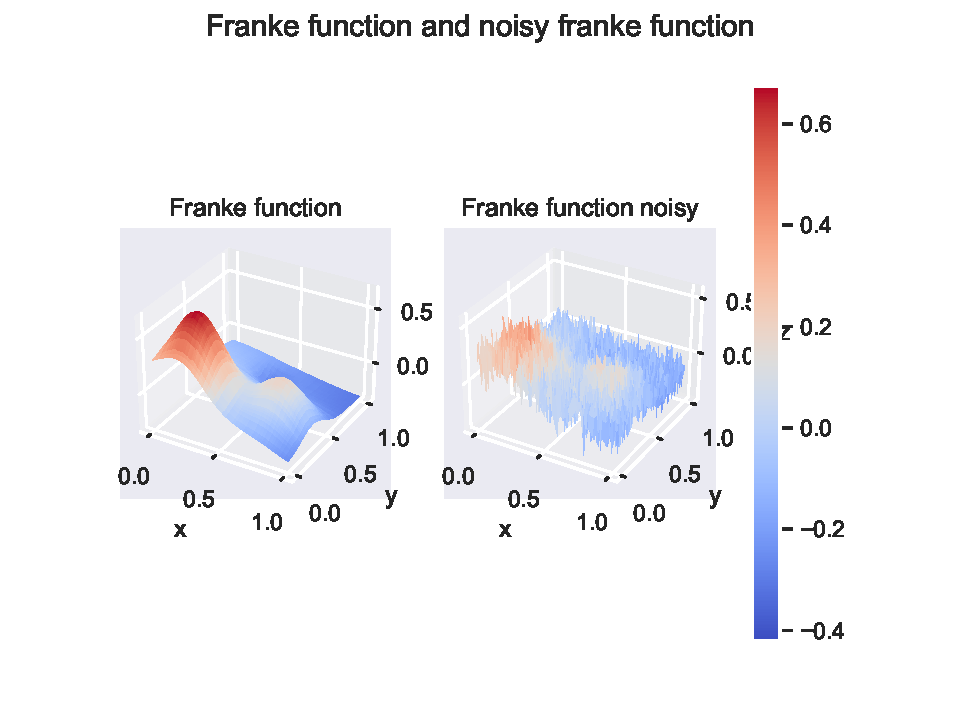
\includegraphics[width=\columnwidth]{../src/output/franke_preview.pdf}
    \caption{Franke function and a franke function with added noise}
    \label{fig:franke_function}
\end{figure}

One the right hand plot we have added noise. This is done to make the training data more exiting. For this and all other noisy franke functions, the noise was generated from a normal distrubution with $\mu=0$, $\sigma^2=0.2$.
% TODO: Talk bout da noise

\subsubsection{Real world terrain data}

The second data that will be used in this article is real world terrain data from an area in Norway. % TODO: WHERE?

In this case we do not have an analytical solution, to generate more data from, like we did for the franke function.

It might seem strange that fitting a model to resemble the terrain data would have any practical advantages.
Why would one want a model which is likely futher from the trut than the real data?

One reason could be to represent the terrain more efficiently. Instead of saving $1800 \cdot 3000=x$, we would only need to save the betas, saving a lot of storage space.   % TODO: Fix dimension

Another reason why doing this regression analysis could be useful, would be if we wanted to approximate the height for locations not directly measured by the real world data captre.

% TODO: Why have we used such little data?

\begin{figure}[H]
    \centering
    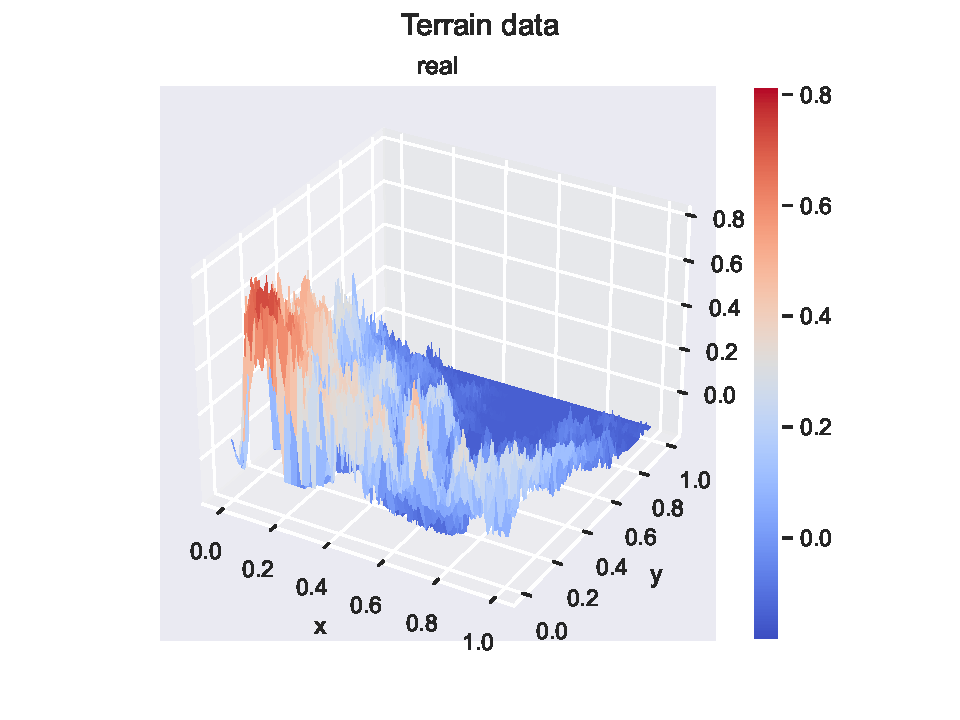
\includegraphics[width=\columnwidth]{../src/output/terrain_preview.pdf}
    \caption{log-log plot of relaxed fixed point iterations}
    \label{fig:terrain_function}
\end{figure}

\subsection{Regression methods}

\subsubsection{Ordinary least squares}

The ordinary least squares was implemented by translating the expression \eqref{eq:optimal_beta_ols} from mathematical notation to a numpy implementation in python.

Assuming that we have a design matrix $X$ and the observed values $z$, we calculate the betas from the following code

\begin{lstlisting}[language=python]
hessian = X.T @ X
hessian_inv = np.linalg.pinv(hessian)
self.beta = hessian_inv @ X.T @ z
\end{lstlisting}

A notable change from the mathematical notation to the code, is that we have used a pseudo-inverse implementation the matrix inversion, as opposed to a mathematical approach, for example using row reduction.
The reason for this change is since we are not guaranteed that our hessian matrix is invertible.
Another possibility would be to check the determinant, but since this requires substantially more computations than just pseudo-inversing it, I have choosen to go for this approach.

\subsubsection{Ridge}

The implementation of ridge regression was pretty similar to that of the OLS-implementation.
The only difference between the OLS and ridge when computing $\bbeta$, was introducting a lambda term.
This means that the OLS-method could have been implemented as a subclass of ridge, with $\lambda=0$.

\begin{lstlisting}[language=python]
hessian = X.T @ X
lambda_I = self.lambda_ * np.identity(len(hessian))
hessian_and_regularized = hessian + lambda_I
hessian_and_regularized_inv = np.linalg.pinv(hessian_and_regularized)
self.beta = hessian_and_regularized_inv @ X.T @ z
\end{lstlisting}

\subsubsection{Lasso}

The OLS-regression and ridge regression were implemented in a pretty similar manner.
Such is not the case also for the lasso-implementation.
The main reason for this is since both the OLS and ridge have closed form expressions for the $\bbeta$, whereas lasso does not.

Therefore, I have choosen to use the already implemented lasso version from scikit-learn.

\subsubsection{Prediction}

Where the fitting procedure was different for the three methods, the predictions were a lot more similar.

\begin{lstlisting}[language=python]
z_tilde = self.beta @ X.T
\end{lstlisting}

\section{Results and discussion}

\subsection{Ordinary least squares}

\subsubsection{MSE and R2}

\begin{figure}[H]
    \centering
    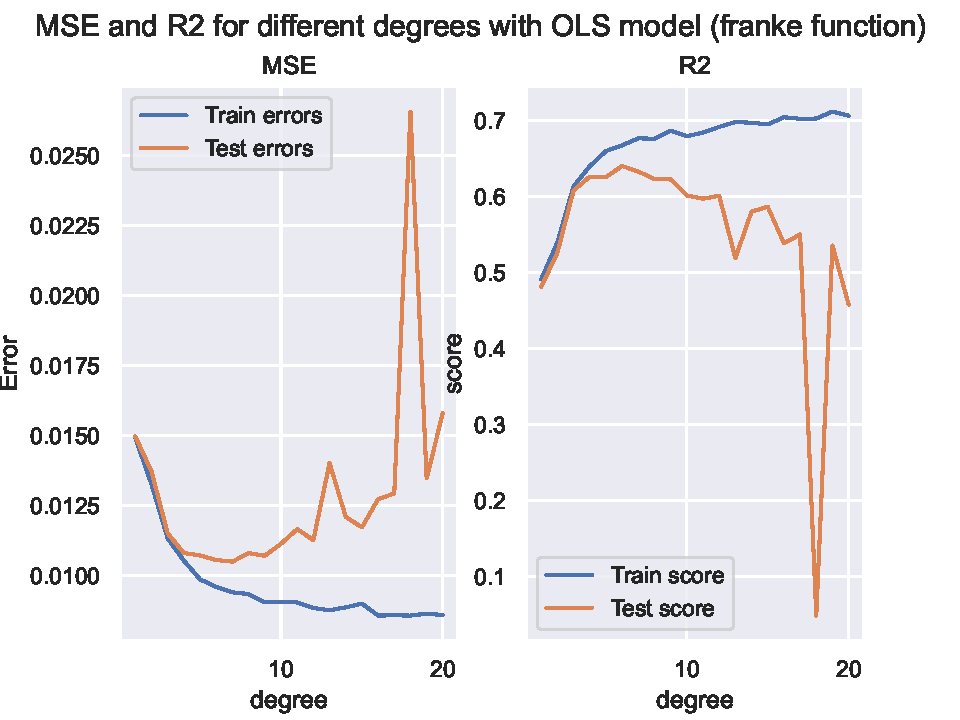
\includegraphics[width=0.8\columnwidth]{../src/output/ols_mse_r2_franke_function.pdf}
    \caption{The MSE and R2 performace of a OLS-models of different degrees trained on data from the franke function and ran for 100 iterations per degree}
    \label{fig:ols_mse_r2_franke}
\end{figure}

\begin{figure}[H]
    \centering
    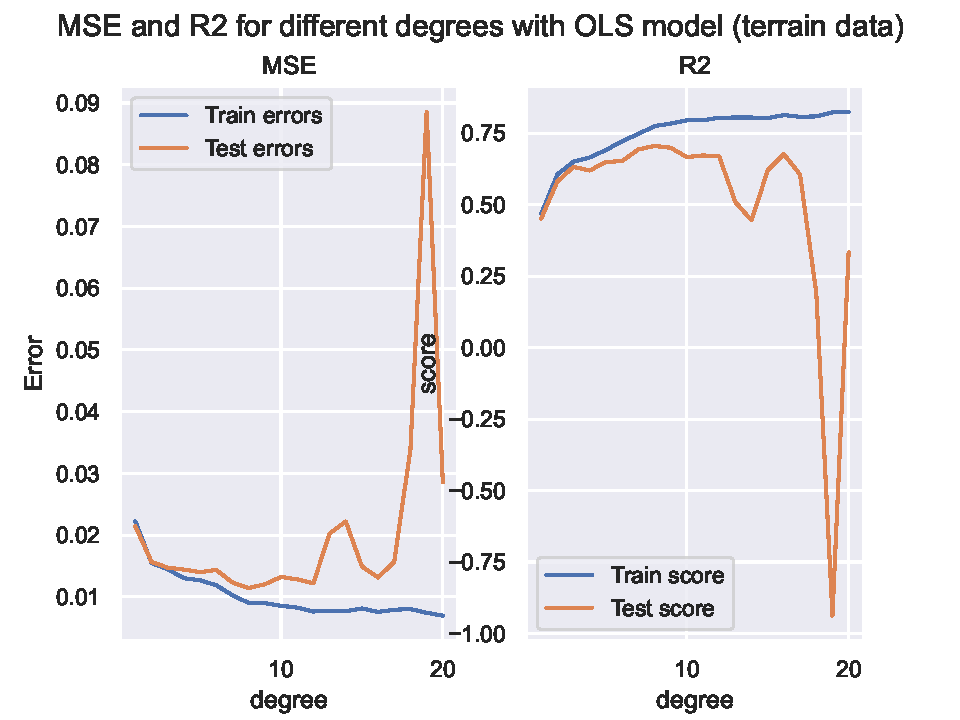
\includegraphics[width=0.8\columnwidth]{../src/output/ols_mse_r2_terrain_data.pdf}
    \caption{The MSE and R2 performace of a OLS-models of different degrees trained on data from the terrain data and ran for 100 iterations per degree}
    \label{fig:ols_mse_r2_terrain}
\end{figure}

We see from both the MSE and R2 plots from both the franke function data and the real world terrain data that for low degrees (up to around 5), the train and test-errors seemed to follow a rather similar path.

When we get to higher degrees that those however, they start to diverge, with much worse performance on the test data, as compared to the training data.

We see that this is especially prominent for degrees bigger than 15.

Another takeaway from the plots, is that we do not always see a decrease in train error as the degree was increased.

If we had used the exact same data for training each time, this would have been the case for the the MSE, since the ordinary least sqares method optimizes for decreasing the MSE.
The reason we sometimes see small increases in train-error, is because we have not used the same data for training each time. To get a more general picture of what increasing the degree did to the data, both algorithms were ran 100 times per degree. This was to avoid having a lucky or unlucky value which impacted the MSE or R2 majorly.

We also see that the performance for the terrain data and data from the franke function follow pretty similar trajectories.
We are using about equal amount of data from both sources, meaning this might explain them following such similar curves.

% Another key takeaway is that the R2 scores generally increase for the training data, when we increase the degree.
% Considering that the R2 score is supposed to explain the fit of the model given the data, it might not be optimal that the R2 score seems to increase.
% Therefore, adjusted R2 scores are sometimes used. % TODO: source, is this wanted?


\subsubsection{Confidence intervals}

\begin{figure}[H]
    \centering
    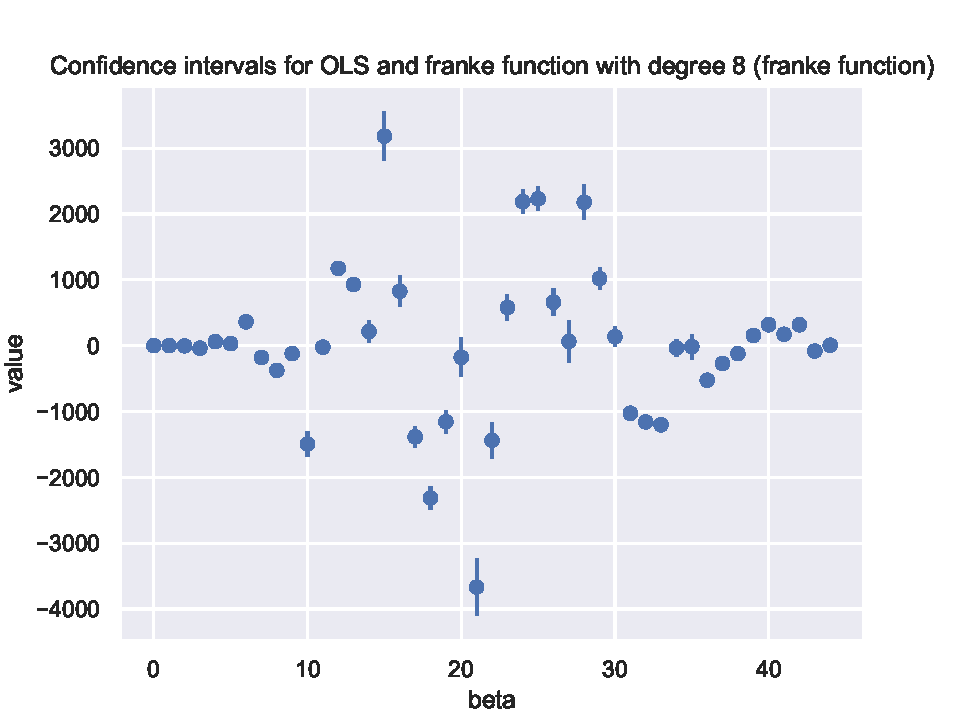
\includegraphics[width=0.8\columnwidth]{../src/output/ols_confidence_intervals_franke_function.pdf}
    \caption{Confidence intervals for different betas from an OLS-model of degree 8 trained on data from the franke function}
    \label{fig:ols_confidence_intervals_franke}
\end{figure}

From the above plot, we see both the values for different betas, with the lines marking the $95\%$ confidence intervals.
Here wee see that many of the first and last betas have small confidence intervals, while the betas in the middle have much higher confidence intervals.

Considering that many of the middle values also have higher or smaller values as compared to the betas on the sides, it seems that the middle betas might both have more impact on the predictions, which might also explain the longer confidence bands.
They are simply there because these variables hold most of the predictive power and thus also are the values we are the least sure are exactly correct.

\begin{figure}[H]
    \centering
    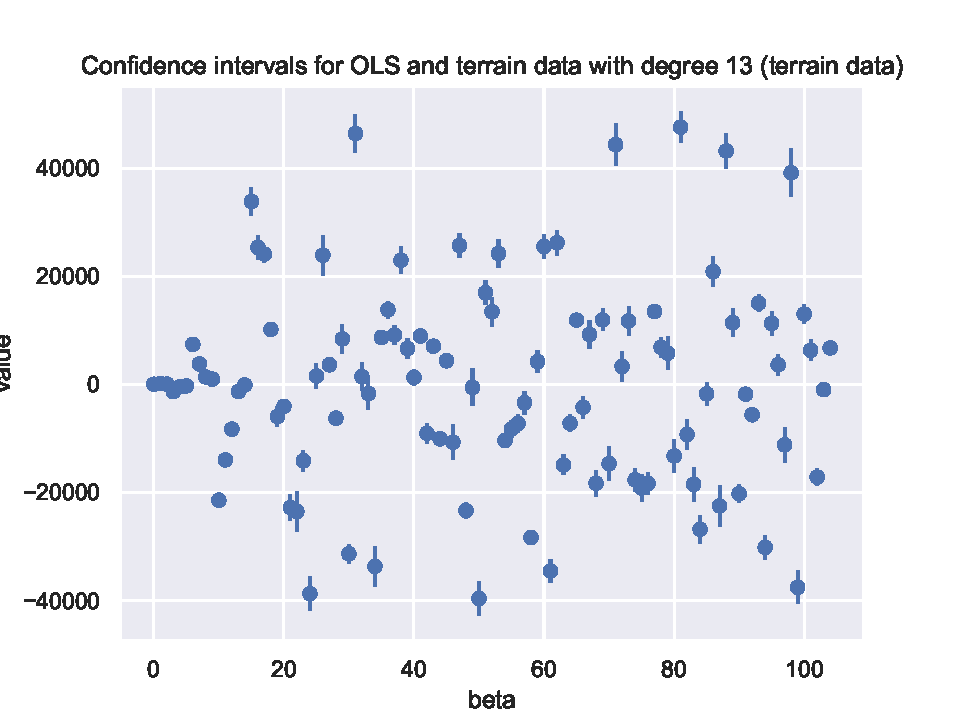
\includegraphics[width=0.8\columnwidth]{../src/output/ols_confidence_intervals_terrain_data.pdf}
    \caption{Confidence intervals for different betas from an OLS-model of degree 8 trained on data from the terrain}
    \label{fig:ols_confidence_intervals_terrain}
\end{figure}

The betas and confidence intervals for ols for the terrain data seem to be pretty spread out, also for the last beta-values.
We also have a higher degree, degree 13 as compared to degree 8 for the OLS.
Considering we are also trying to fit different data, it is natural that the beta-values for the two different plots are quite different.

Another clear difference is that the betas of the terrain data have much higher values.
This means that even tough the confidence intervals might seem to be smaller for the terrain data, we cant know for certain using only the plots.

% TODO: Note that the reason for different degrees were since the optimal degree were better
% TODO: Check the analytical difference between the terrain and the frank in confidence interval size

\subsection{Bias-variance trade-off}

\begin{figure}[H]
    \centering
    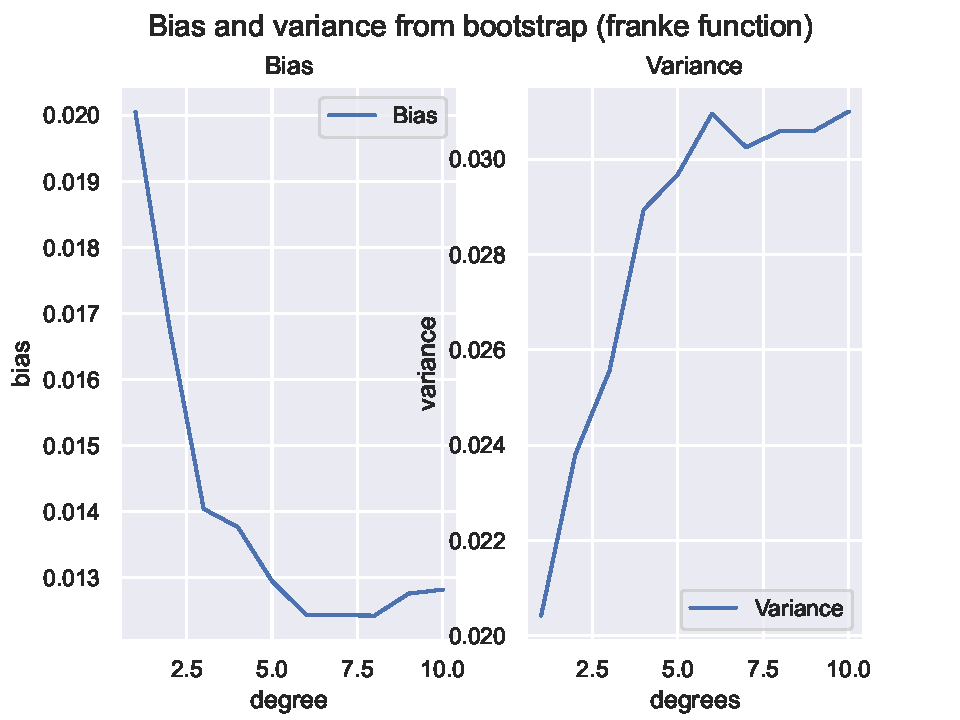
\includegraphics[width=0.8\columnwidth]{../src/output/bootstrap_bias_variance_franke_function.pdf}
    \caption{Bias and variance curves obtained using bootstrap with an OLS-model for franke function data}
    \label{fig:franke_bias_variance_bootstrap}
\end{figure}

In general, the bias seems to decrease when we increase the degree for the OLS method, while the variance increases.
These observations are in tune with the theory.
That said, these are not as nice as those found in text books, where there is a clear optimal degree where both the bias and variance are low.

From the plot we see that the bias seems to decrease as the variance increases, with both changing fast up to degree 3, and stabilizing after that.

From earlier plots, we remember that we minimized test MSE for the OLS on data from the franke function at degree 8.

According to this figure, that means that we will have lower bias but higher variance.

\begin{figure}[H]
    \centering
    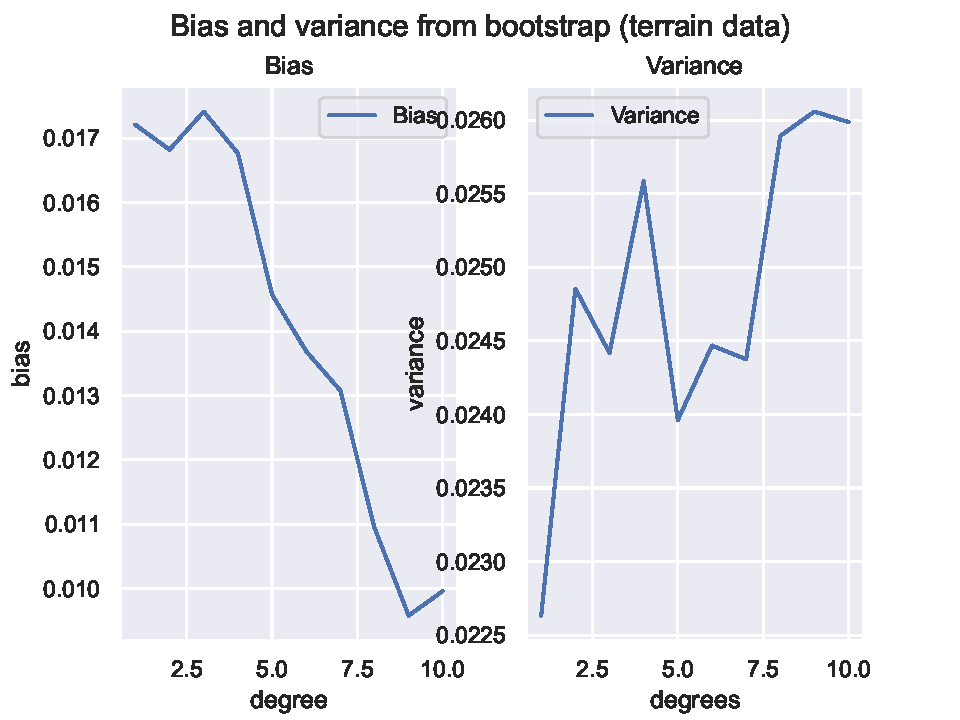
\includegraphics[width=0.8\columnwidth]{../src/output/bootstrap_bias_variance_terrain_data.pdf}
    \caption{Bias and variance curves obtained using bootstrap with an OLS-model for terrain data}
    \label{fig:terrain_bias_variance_bootstrap}
\end{figure}

For the terrain data, the graphs seem to behave a bit differently than Fig \ref{fig:franke_bias_variance_bootstrap}, with a less stable trend, especially for the variance.
The bias, however, seems to become smaller and smaller as the degree increases, which is more understandable.

The reason for the variance being ustable, might be because the terrain data seems to be more complex than the franke data, thus meaning this might have been one of the reasons why it is unstable, since none of the are actually able to capture the real data, and therefore get more variance from degree to degree.

% TODO: Discuss the use of the bias-variance trade-off

\subsection{Cross-validation}

% TODO: Compare my k-fold cv to the scikit-learn one?

\begin{figure}[H]
    \centering
    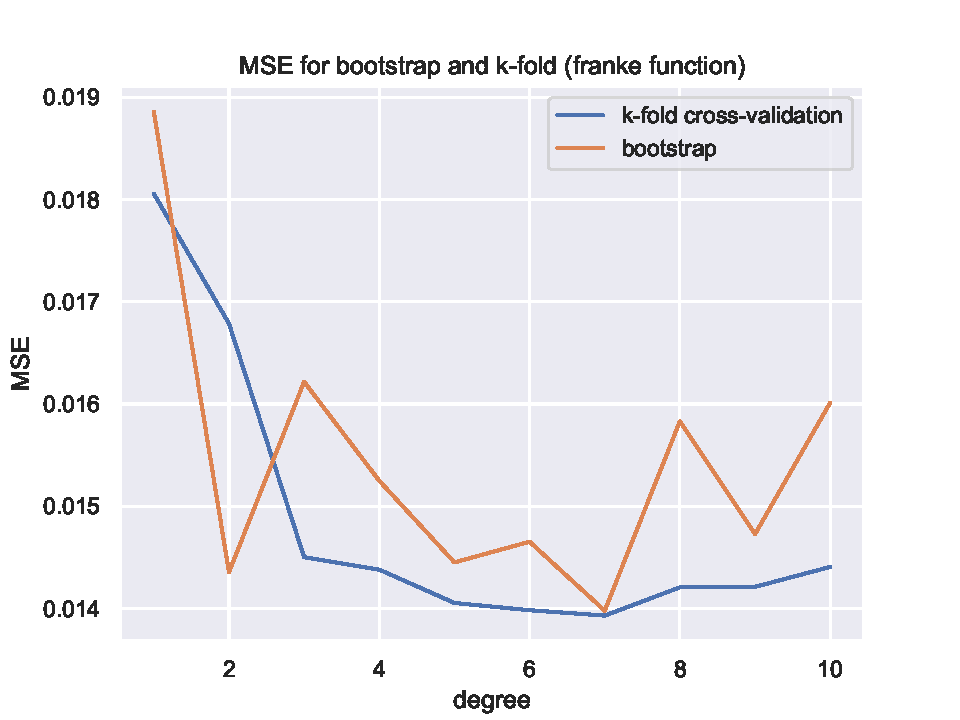
\includegraphics[width=0.7\columnwidth]{../src/output/bootstrap_cross_validation_franke_function.pdf}
    \caption{MSE estimate from k-fold cross-validation compared to a bootstrap method for data from the franke function}
    \label{fig:bootstrap_cross_validation_franke}
\end{figure}

\begin{figure}[H]
    \centering
    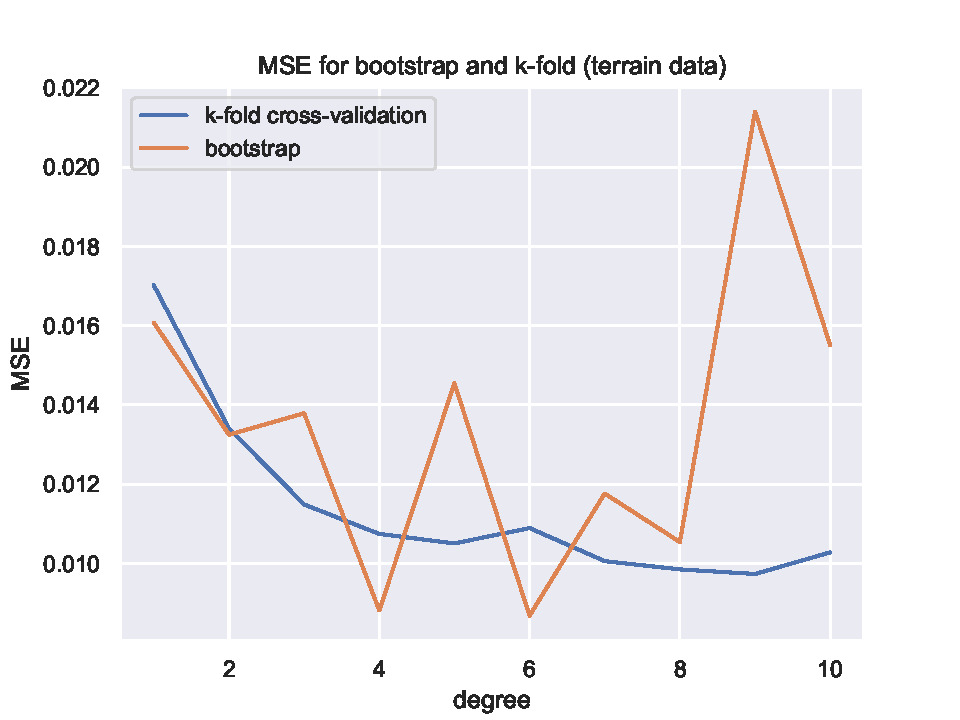
\includegraphics[width=0.7\columnwidth]{../src/output/bootstrap_cross_validation_terrain_data.pdf}
    \caption{MSE estimate from k-fold cross-validation compared to a bootstrap method for data from the terrain data}
    \label{fig:bootstrap_cross_validation_terrain}
\end{figure}

We see that the MSE from the k-fold cross-validation and the bootstrap follow some of the same trends, but the bootstrap method seems to have more variance from degree to degree.

One of the reasons for this might be because we for the k-fold cross-validation use all of the data for predicting MSE at some point, while we for the bootstrap use the same data multiple times.
This means that if for instance one of the values is a very bad for for the model, this might cause a big difference in MSE, while this value likely will have less impact on the cross-validation, since the model is fitted differently each time and thus has a bigger change of sometimes fitting also this value.

\subsection{Ridge}

\begin{figure}[H]
    \centering
    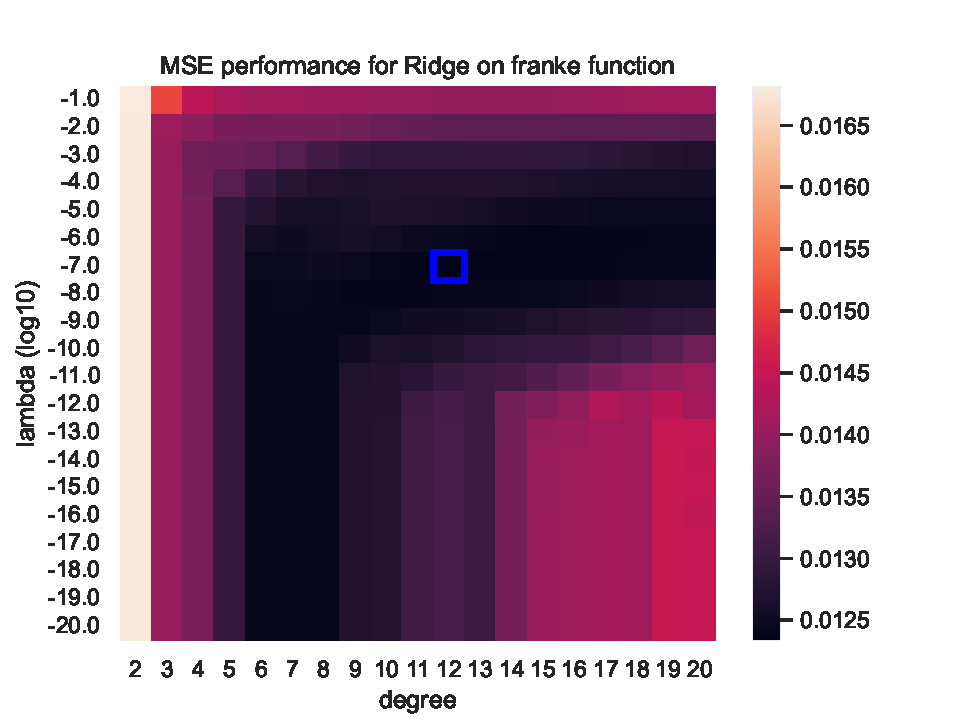
\includegraphics[width=0.8\columnwidth]{../src/output/mse_heat_plot_franke_function_Ridge.pdf}
    \caption{A heat plot for the MSE performance for different lambda values and degrees for fitting a ridge model, with the blue square marking the best performance for data from the franke function}
    \label{fig:mse_heat_map_franke_ridge}
\end{figure}

\begin{figure}[H]
    \centering
    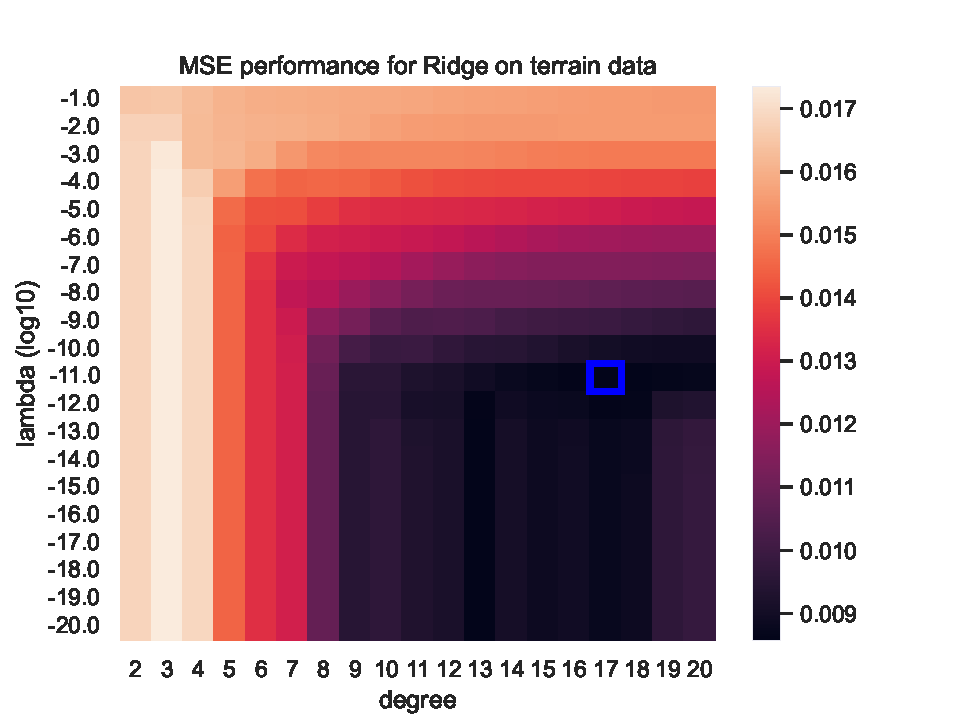
\includegraphics[width=0.7\columnwidth]{../src/output/mse_heat_plot_terrain_data_Ridge.pdf}
    \caption{A heat plot for the MSE performance for different lambda values and degrees for fitting a ridge model, with the blue square marking the best performance for data from the terrain data}
    \label{fig:mse_heat_map_terrain_ridge}
\end{figure}

For the ridge regression, we not only need to find a degree which yields a small MSE, we also need to find a good lambda-value.

This means that we are no longer to plot the performance in a line plot, like we could do for the OLS.
I have therefore opted for a heat plot. That means that both the x- and the y-axis specify different degrees and lambdas, while the color specifies the errors.

% TODO: More discussion here?

\subsection{Lasso}

\begin{figure}[H]
    \centering
    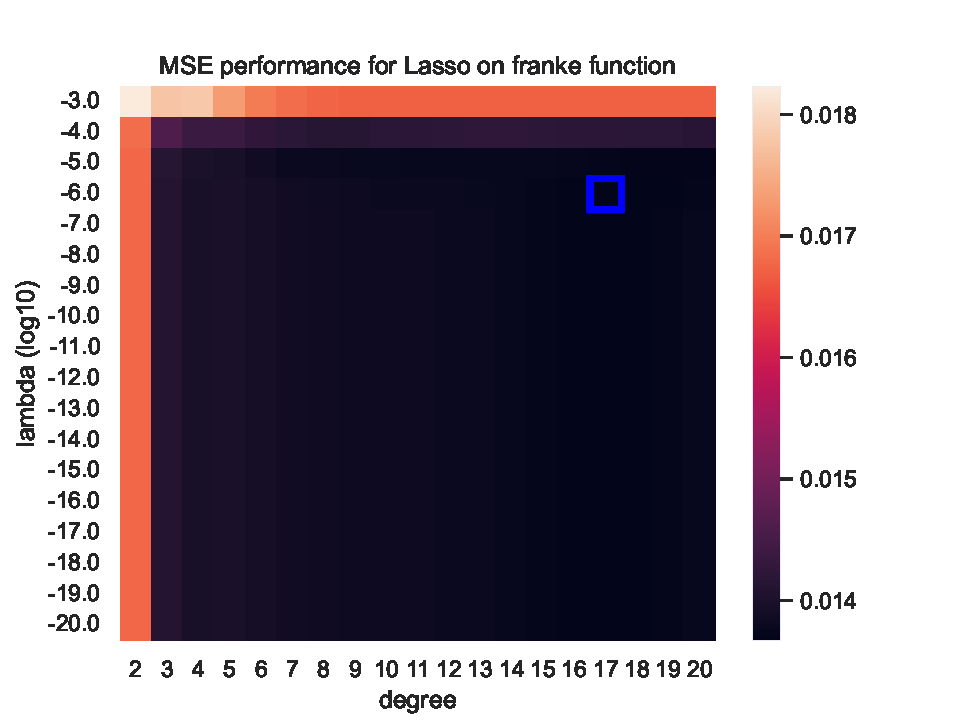
\includegraphics[width=0.65\columnwidth]{../src/output/mse_heat_plot_franke_function_Lasso.pdf}
    \caption{A heat plot for the MSE performance for different lambda values and degrees for fitting a lasso model, with the blue square marking the best performance for data from the franke function}
    \label{fig:mse_heat_map_franke_lasso}
\end{figure}

\begin{figure}[H]
    \centering
    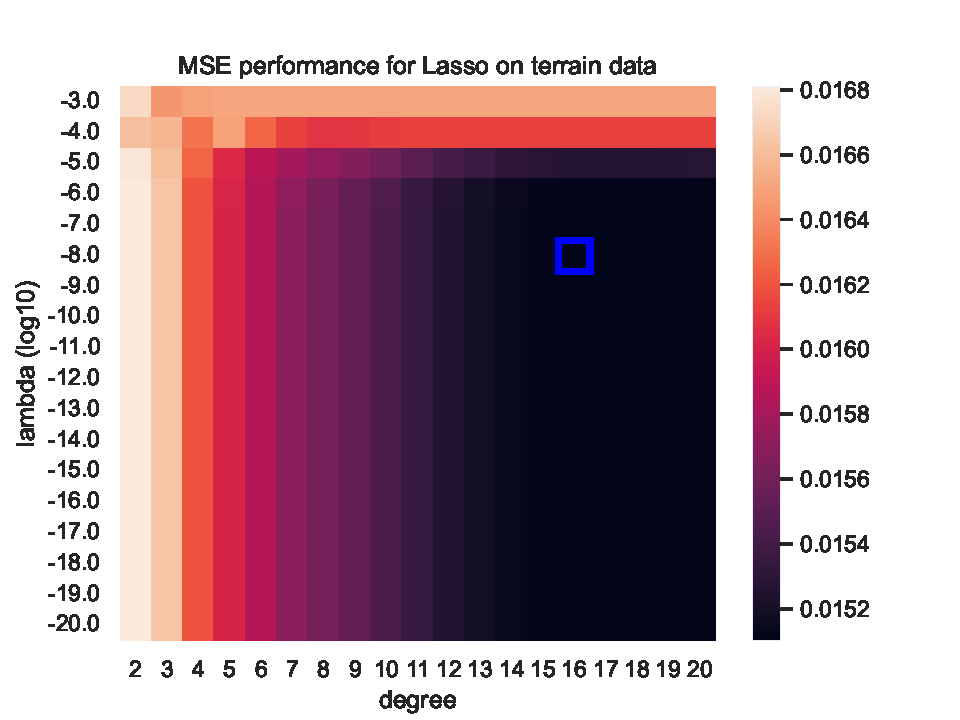
\includegraphics[width=0.65\columnwidth]{../src/output/mse_heat_plot_terrain_data_Lasso.pdf}
    \caption{A heat plot for the MSE performance for different lambda values and degrees for fitting a lasso model, with the blue square marking the best performance for data from the terrain data}
    \label{fig:mse_heat_map_terrain_lasso}
\end{figure}

The lasso plots can be interpreded by the same manner as the ridge regression.

% TODO: DISCUSS BETTER
Something notable is that the lasso seems to be more stable for different values of lambda, with pretty even colors, whereas for the ridge, there are different colors for different lamdbas, for the same degree.

\subsection{Predictions}

After doing the analysis and obtaining the optimal parameters from MSE test-scores. We can finally use the values to predict on the data.

\begin{figure}[H]
    \centering
    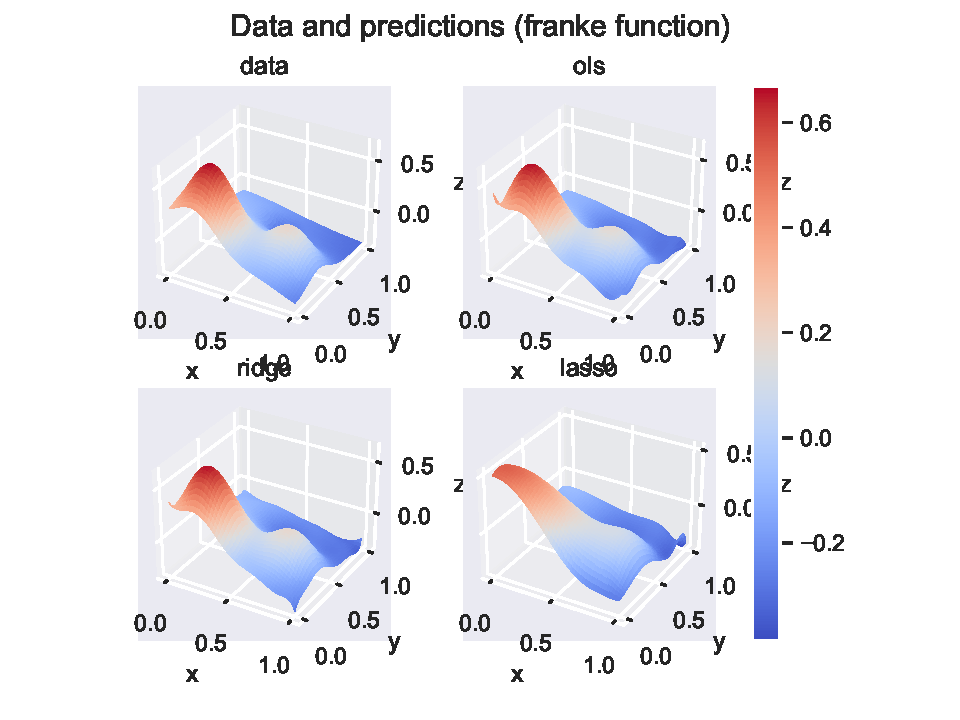
\includegraphics[width=\columnwidth]{../src/output/prediction_all_models_franke_function.pdf}
    \caption{Prediction for the best parameters obtained for the ols method, ridge regression and lasso regression for the franke function}
    \label{fig:predictions_franke_function}
\end{figure}
% TODO: Fix the sizing of the plots
We see that the our predicted models were pretty close to the real data from the franke function, especially the ridge and the ordinary least squares seem to fit teh data pretty closly.
We see that the lasso model has fewer curves than the other two models.
This means that even tough it might not fit as close to the train data, it might in some cases be able to generalized better.

% MSE OLS: 
% MSE RIDGE: 
% MSE LASSO: 

\vspace{0.5em}
\begin{tabular}{ |p{3cm}||p{6cm}|  }
 \hline
 \multicolumn{2}{|c|}{Mean squared error franke function} \\
 \hline
 OLS & 0.00020860008434628492  \\
 \hline
Ridge & 0.000123860308040720\\
\hline
Lasso  & 0.003175374379351624\\
\hline
\end{tabular}

\vspace{0.5em}

From the table we see that the ridge regression method clearly has the best performance, with the ordinary least squares in second and lasso performing quite a lot worse.

\begin{figure}[H]
    \centering
    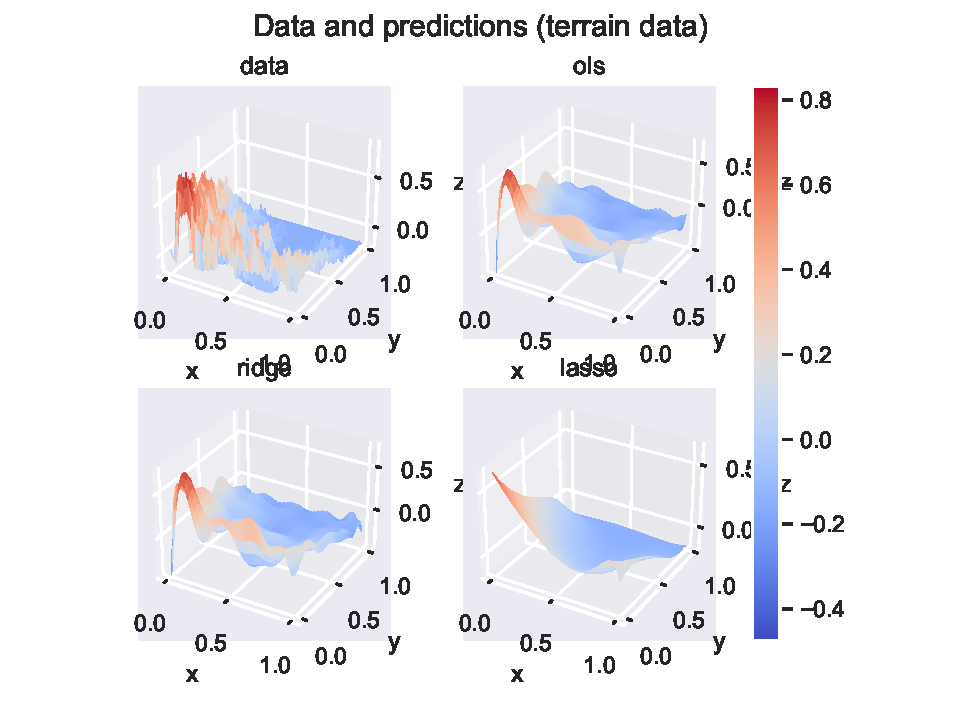
\includegraphics[width=\columnwidth]{../src/output/prediction_all_models_terrain_data.pdf}
    \caption{Prediction for the best parameters obtained for the ols method, ridge regression and lasso regression for the terrain data}
    \label{fig:predictions_terrain_data}
\end{figure}

The terrain data has a more caotic structure.
We see that both the ols and ridge again seem to fit closer to the real data as compared to the lasso.

\vspace{0.5em}
\begin{tabular}{ |p{3cm}||p{6cm}|  }
 \hline
 \multicolumn{2}{|c|}{Mean squared error terrain data} \\
 \hline
 OLS & 0.007826979500050183  \\
 \hline
Ridge & 0.007519375592550991 \\
\hline
Lasso  & 0.011560616105923953 \\
\hline
\end{tabular}

\vspace{0.5em}
We again see that the ridge regression model has the best performance one again, but this time it is pretty close between the OLS and the ridge, with the lasso model coming not that far behind.


\section{Conclusion}

The goals of this project was to explore different methods for doing linear regression, more specifically looking at the performance of the ordinary least squares, ridge regression and lasso regression.
We also wanted to get a better understanding of other consepts central to machine learning, like train/test splitting, bootstrap and cross validation.

From the testing on the two dataset the ridge regression method seems to be performing the best, with ordinary least squares in second.
The lasso method performed the worse, seeming unable to fit more complex data. 

These results should not ble trusted blindly.
One major potential drawback with my testing, is limited computational power.
When trying to fit a lasso model on all the terrain data, it used more than three hours of cpu time, to fit a single value.
This means that it was fitted only on a small portion of the data.

I could have also done other tests, for example testing more extensivly different distributions of test/train size, different amounts of noise or testing for different data sizes.
Using the franke function, it would have been very easy to look at differences between the performance of models with much and little data.

The lasso model also seemed no not be able to fit the data closely enough.
Given a more powerful computer, I could have probably tried trainig for higher degrees, maybe leading to finding an even better fit.



% TODO: Discussion:
% could have varied the N, especially for the franke



\section{Appendix}

\subsection{Code}

The code is on github, with a more detailed explenation on the github README page and the docstring for the different functions.

\subsection{Bias-variance tradeoff}

\begin{align*}
 & E\left((f - \tilde{y})^2\right) \\
 &   = E\left((f+\varepsilon - \tilde{y} )^2\right) \\
 &   = E\left((f+\varepsilon - \tilde{y} +E(\tilde{y})-E(\tilde{y}))^2\right) \\
 &   = E\left((f-E(\tilde{y}))^2\right)+E(\varepsilon^2)+E\left((E(\tilde{y})- \tilde{y})^2\right) \\
 &   \quad  +2E\left((f-E(\tilde{y}))\varepsilon\right)
+2E\left(\varepsilon(E(\tilde{y})- \tilde{y})\right)
+2E\left((E(\tilde{y})- \tilde{y})(f-E(\tilde{y}))\right) \\
 &   = (f-E(\tilde{y}))^2+E(\varepsilon^2)+E\left((E(\tilde{y})- \tilde{y})^2\right) 
+2(f-E(\tilde{y}))E(\varepsilon) \\
 &   \quad +2E(\varepsilon)E\left(E(\tilde{y})- \tilde{y}\right)
 +2E\left(E(\tilde{y})- \tilde{y}\right)(f-E(\tilde{y})) \\
 &   = (f-E(\tilde{y}))^2+E(\varepsilon^2)+E\left((E(\tilde{y})- \tilde{y})^2\right)\\
 &   = (f-E(\tilde{y}))^2+Var(\varepsilon)+Var\left(\tilde{y}\right)\\
 &   = Bias(\tilde{y})^2+\sigma^2+Var\left(\tilde{y}\right)\\
\end{align*}

\begin{thebibliography}{9}
\bibitem{texbook}
T. Hastie, R. Tibshirani, and J. Friedman.
\emph{The Elements of Statistical Learning: Data Mining, Interference, and Prediction, Second Edition.} Springer Series in Statistics. Springer New York, 2009. ISBN: 9780387848587

\bibitem{lecture notes two}
Hjorth-Jensen, M. \emph{Lecture notes}, FYS-STK4155, 2021, \url{https://compphysics.github.io/MachineLearning/doc/LectureNotes/_build/html/intro.html}

\bibitem{lecture notes one}
Hjorth-Jensen, M. \emph{Lecture notes}, FYS-STK4155, 2021, \url{https://compphysics.github.io/MachineLearning/doc/web/course.html}

\bibitem{webpage}
EarthExporer, https://earthexporerer.usgs.gov, data downloaded to ../src/data/geodata.tif

\end{thebibliography}

\end{document}
